\documentclass{myproc}
%\addtolength{\topmargin}{-2cm}
%\addtolength{\textheight}{2cm}
\usepackage{mathptm,mydef}
\usepackage{graphicx}
\DeclareGraphicsExtensions{.png,.jpg}
%\usepackage{courier}
\usepackage{epsfig}
\usepackage{alltt}
\usepackage[T1]{fontenc}
%\renewcommand{\ttdefault}{txtt}
\usepackage[all]{xy}
%\usepackage{MinionPro}

\usepackage{hyperref}
\hypersetup{
    colorlinks, 
    citecolor=black, 
    filecolor=black, 
    linkcolor=blue, 
    urlcolor=black
}

\begin{document}
\small


\begin{center}
{\large\bf SmartThings: Overview}
\end{center}

\vspace*{1cm}

\tableofcontents

%\pagebreak

\section{Overview}
\bit
\w \bb{Target domain}: Home automation
\w \bb{devices} provide native capability
\w \bb{composition of native device services} happen at \bb{CLOUD}, FOR NOW!
  \bit
  \w they are thinking of moving some capability (i.e intelligent logic or
  choreography code to Hubs) 
  \w c.f. Meadow is flexible enough to put ``composition logic'' into
  anywhere (cloud, hub, or device itself). 
  \eit
\eit

\subsection{Physical graphs}
\bit
\w SmartThings: \textcolor{red2}{\bb{platform for ``Open Physical Graph''}}
\w \bb{physical graph}: virtual, online representation of physical world
\w people interact with physical graph
\w graphs are dynamic -- nodes come and go, users can perceive dynamicity of
graphs 
\w graph is hierarchical -- graph of graphs, etc.
\w nodes/devices can be \bb{manipulated} and are \bb{programmable}
\eit

\subsection{What they believe}
\bit
\w \bb{They believe that intelligence (some reactive code) should be separated
from devices ==> put in CLOUD or HUB!}
\eit

\section{Architecture}

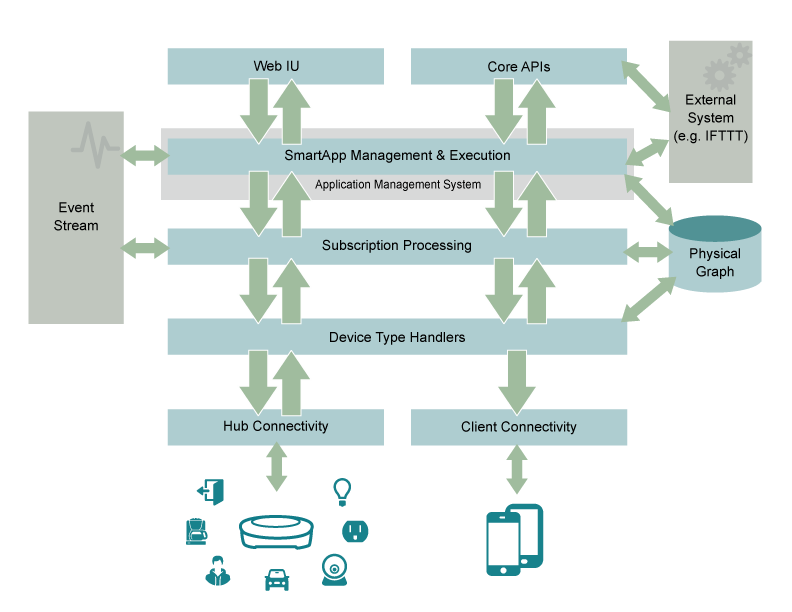
\includegraphics[width=9cm]{pics/arch}

\subsection{Components}
\bit
\w \textcolor{red2}{\bf{end-devices}}: connected to SmartThings Hub
  (e.g. ZigBee devices) or directly connected to Cloud (e.g. devices which
  directly connected to TCP/IP)
\w \textcolor{red2}{\bf{SmartThings Hub}}: network gateway which connects
ZigBee/Z-Wave network to the Internet + some event communination capability
between CLOUD and devices
\w \textcolor{red2}{\bf{SmartThings Cloud}}: centralized server
\w \textcolor{red2}{\bf{User Experience}}: just U/I programs (e.g. iPhone,
Android app) which uses some API which accesses Cloud
\eit

\subsection{SmartThings Cloud Functionalities}
\bit
\w \textcolor{red2}{\bf{connectivity}}: provides connection between Hubs and
Apps
\begin{verbatim}
  devices - (Hubs) - CLOUD - (iPhone) - apps
\end{verbatim}
\w \textcolor{red2}{\bf{device management \& capability abstraction}}:
  \bit
  \w \textcolor{blue2}{some notion we abandoned at early stage}
  \w \textcolor{blue2}{should we create some ``first-class'' treatment of device categories?}
     (e.g. ``switches'' abstract all ``GE switch'', ``logitech switch'', etc.)
  \w \textcolor{blue2}{maybe not a good idea}
  \w \textcolor{blue2}{we may need to provide ``MECHANISM'' but let users to implement
  ``POLICY'' using the meachanism}
  \w \textcolor{blue2}{Some ``overlaying'' tag-based mechanism (e.g. Gmail tag) could be a
  better alternative}
  \eit
\w \textcolor{red2}{\bf{Event processing \& routing}}: event pub/sub layer
   + some limited event processing (filtering, etc.)
  \bit
  \w trivial; rather bland
  \eit
\w \textcolor{red2}{\bf{Applications (SmartApps)}}: just provides some API
which external programs can access cloud
  \bit
  \w trivial
  \eit
\w \textcolor{red2}{\bf{Web services}}: provides the web service API so Web
developers can be used
  \bit
  \w trivial
  \eit
\eit

\subsection{Current status}
\bit
\w Supported protocols: ZigBee, Z-Wave, WiFi, etc.
\w Sells two types of kits:
  \bit
  \w Kit \#1: Only observe device status
  \w Kit \#2: Both observe and control devices
  \eit
\w When service request is sent, ``fire and forget'' (asynchronous call) -- no
   service guarantee  
\w cloud-based: \bb{centralized server}
\eit
\subsection{Future plan}
\bit
\w from cloud to distributed hub-based
\w support blocking service request
\eit


\section{How They Support Adding Smartness}
\bit
\w \textcolor{red2}{\bf{device-type handlers}}:  some sort of ``device
driver'' which connects physical device and the ``SmartThings world''
   \bit
   \w \textcolor{blue2}{\bf{}maybe we might need to adopt this idea; so far,
   we have thought about some ``import capability'' to import native device
   capability into Meadow; however, more solid ``abstraction'' is needed}
   \eit
\w \textcolor{red2}{\bf{}event-handler SmartApps}: just some primitive-form of
\textcolor{blue2}{\bf{}Meadow reactors} 
\w \textcolor{red2}{\bf{}Dashboard Solutio Mobile SmartApps}: some U/I tool
   (U/I version of Meadow shell?)
\w \textcolor{red2}{\bf{}Integration SmartApps}: SmartApps can
\textcolor{blue2}{\bf{}use/provide web services}, which means that they would
  provide some runtime which provides services but only in web services form.
  \bit
  \w need to compare our approach (which provides own language)
  \w DISCUSS: is ``web services'' a technology worth pursuing? (losing to REST
  API) 
  \w need to dig futher
  \eit
\eit

\section{Event handlers}

\begin{alltt}
\textcolor{red2}{def contactHandler(evt) \{
  log.debug "\$evt.value"
  if (evt.value == "open") \{
    switch1.on()
  \} else if (evt.value == "closed") \{
    switch1.off()
  \}
\}}
\end{alltt}

\section{Criticisms}
\bit
\w \bb{Hard-coded device types}
\w \bb{Groovy for describing event handlers}
\w \bb{Supporting concurrency}: 
\w \bb{Lack of blocking calls}:
  Supporting blocking calls requires sophisticated scheduling mechanism
  installed inside the ``collective'' runtime.
  Let a single event handler $H$ be executed. They may just schedule one
  Java thread to handle this. When blocking calls are supported, there may be
  huge number of threads pending in the middle (waiting for reponses) -- Java
  thread based scheduling cannot scale.
\eit
\end{document}
